\section{GPR model}\label{GPR}

An introduction of Gaussian Process Regression (GPR) model and the package GPy. What does a GPR model learn from the data and how it predict stellar parameters?  

\subsection{Discussion about kernels}
 The analysing is mainly based on the MLP kernel because data is multiple-demission, and we also use other kernels (Exponential) to combine with the MLP kernel to improve the fitting. 

\subsection{Selection of GPR Model Inputs}
We aim to derive observables from fundamental input parameters of the grid. As mentioned in Section~\ref{sec:grid}, our model grid has five independent fundamental inputs, says, mass, initial metallicity, initial helium fraction, mixing-length parameter, and age. The GPR model inputs are ideally in fixed dynamic ranges (form a cube-like space), however, the age ranges significantly vary on different tracks. We hence define an age index to replace the age as an input, and putted the age as an output. The age index is calculated on each evolutionary track following 
\begin{equation}
 t' = 10^{(t/t_{\rm max})},
\end{equation}
where $t$ is the age, $t_{\rm max}$ is the maximum age of a track. Note that $t_{\rm max}$ must be defined in the same way for all evolutionary tracks. In this work, we defined $t_{\rm max}$ as the age when a track evolve to $\log g$ = 3.8. The purpose to use an exponential formula is flattening sharp changes of observables in the last 10\% lifetime. This make GPR models converge easily. A comparison between GPR models using $t/t_{\rm max}$ and $10^{(t/t_{\rm max})}$ is illustrated in Figure~\ref{fig:selection_of_t}.  As it can be seen that, the effective temperature evolutaion presents a hump around 0.7 of the lifetime (which is the hook) and quickly drops in the last 10\% lifetime (the subgiant phase). The GPR model in the top panel does not well learn these two stages, and the residuals (blue dots in the bottom graph) go up to ±1K. By using $10^{(t/t_{\rm max})}$ as the input, those sharp changes are flattened and hence the GPR model predictions are significantly improved (the maximum residual is down to $\sim10^{4}$ K). We lastly summary our selections of GPR model inputs and outputs as below. 
\begin{itemize}
\item GPR model inputs:
\item[] Mass ($M$ = 0.8 -- 1.2$M_{\odot}$)
\item[] Age index ($t'$ = 0.0 -- 10)
\item[] Initial metallicity ([Fe/H]$_{\rm init}$ = -0.5 -- 0.5)
\item[] Initial helium fraction ($Y_{\rm init}$ = 0.24 -- 0.32)
\item[] Mixing-length parameter ($\alpha_{\rm MLT}$ = 1.7 -- 2.3)
\item GPR model outputs: 
\item[] Effective temperature ($T_{\rm eff}$) 
\item[] Surface gravity ($\log g$)
\item[] Radius ($R$)
\item[] Surface metallicity ([Fe/H])
\item[] Two global seismic parameters ($\Delta\nu$ and $\nu_{\rm max}$)  
\end{itemize}
Thus, our GPR model can be described as 
\begin{equation}\label{gprmodel}
{\rm Observables} = f(M, t', ({\rm Fe/H})_{\rm init}, Y_{\rm init}, \alpha_{\rm MLT}). 
\end{equation}

\begin{figure}
	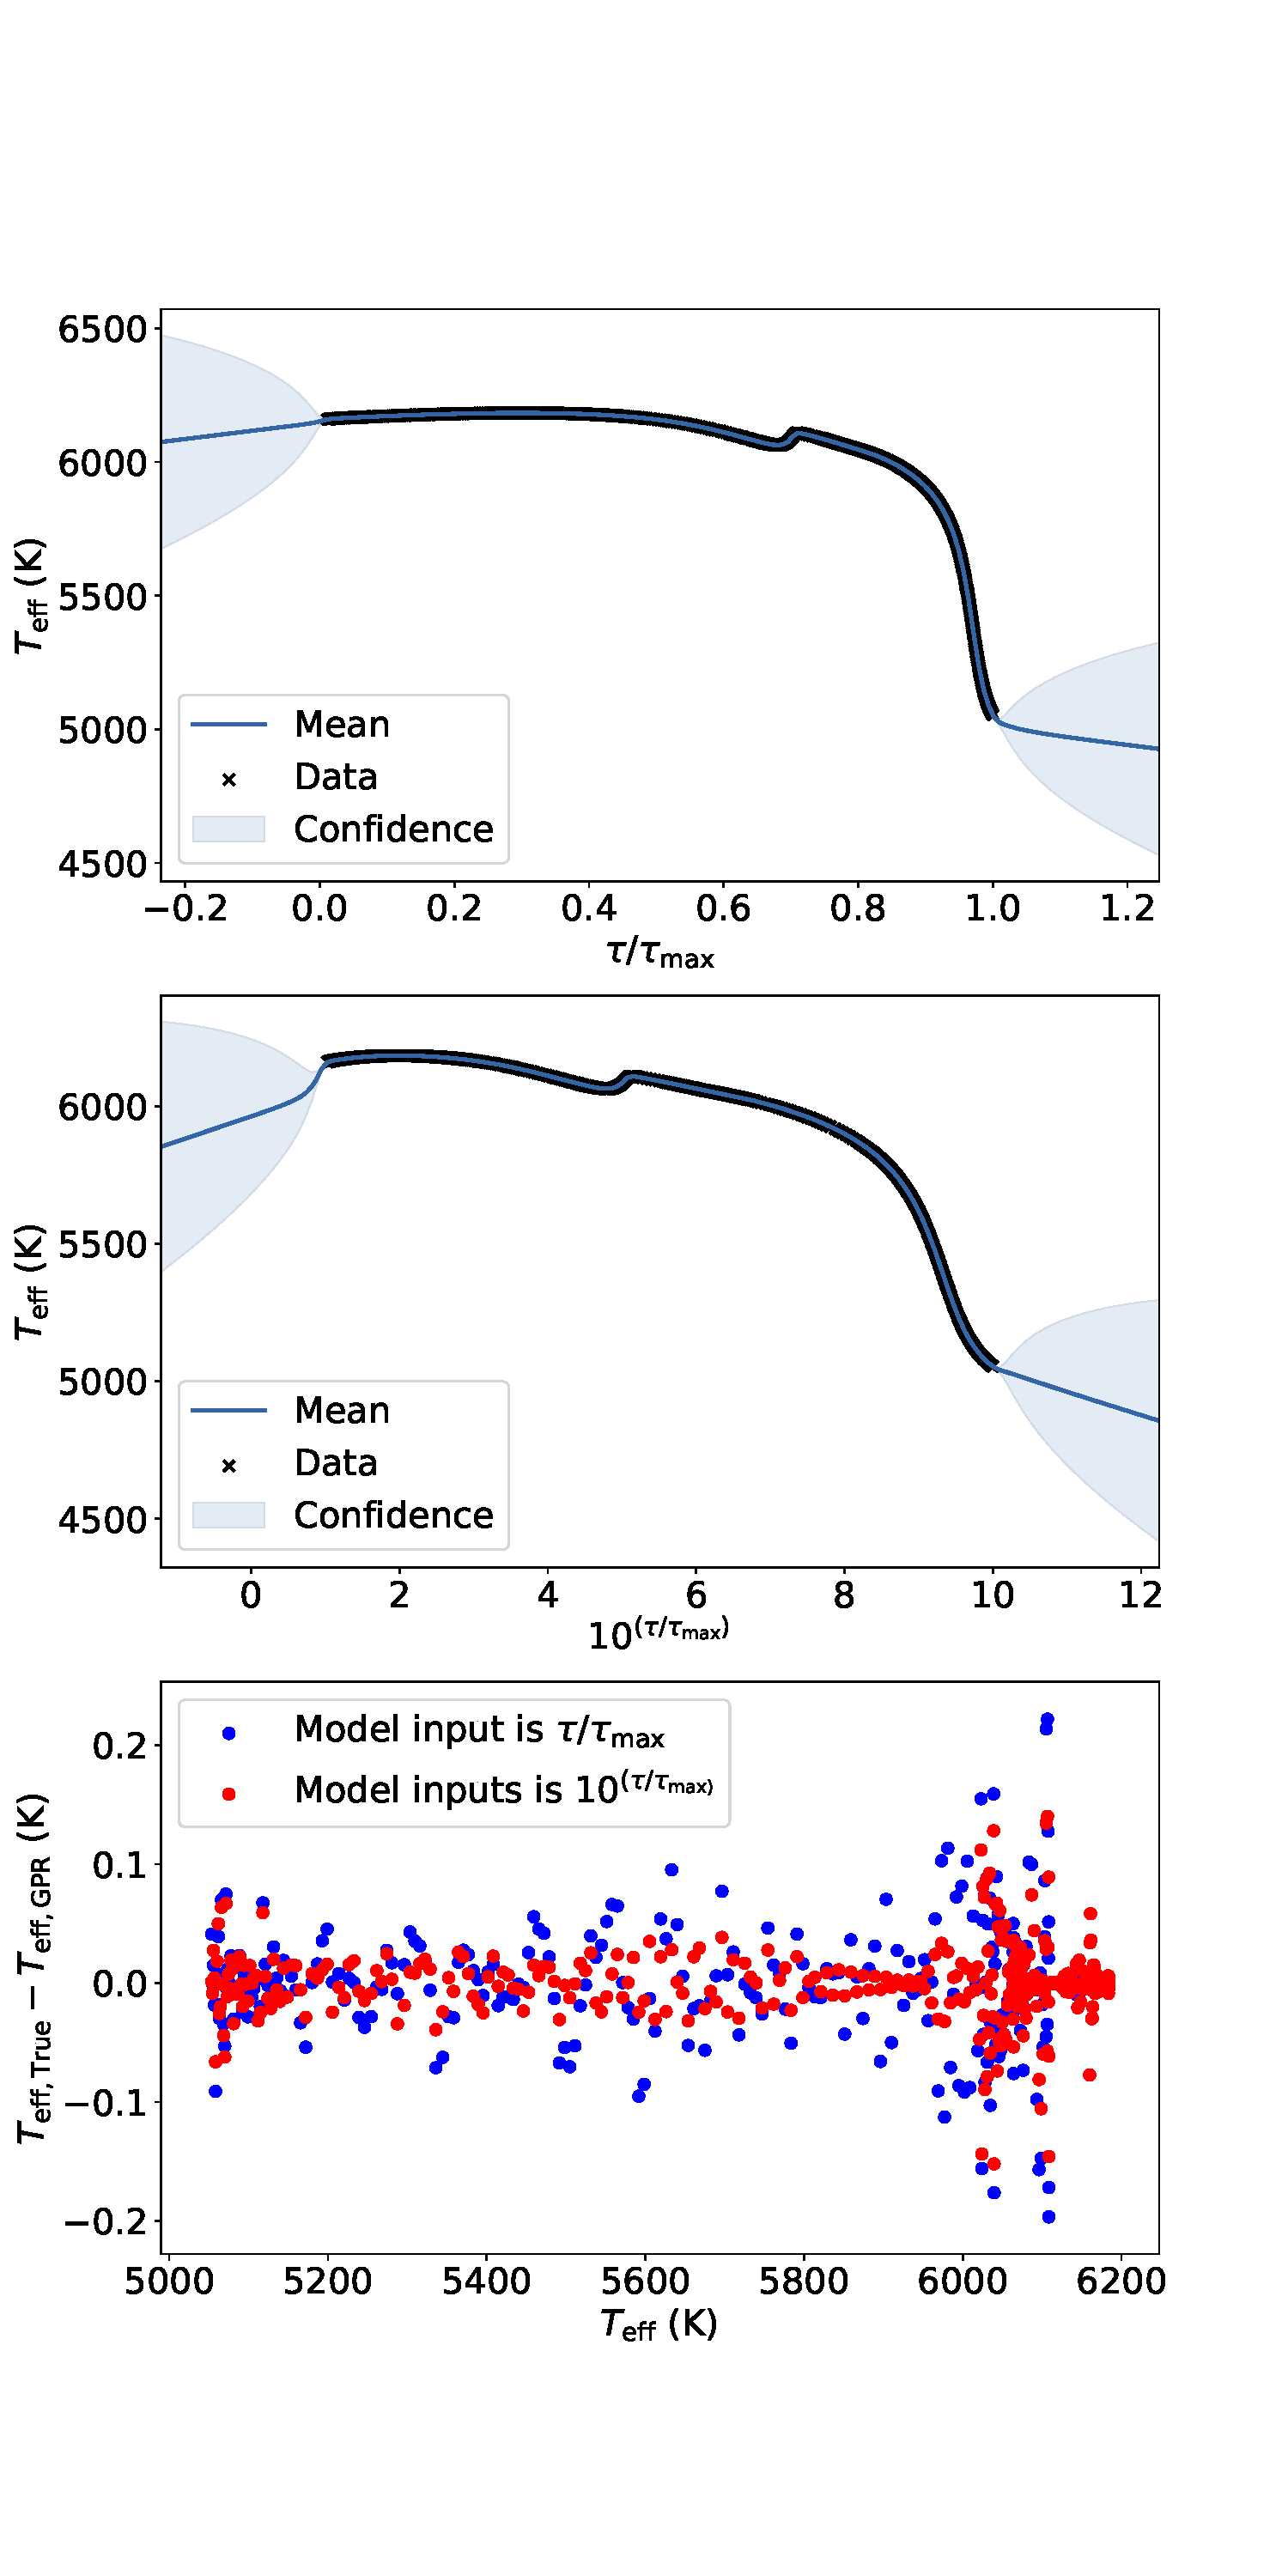
\includegraphics[width=1.0\columnwidth]{selection_of_t.pdf}
    \caption{The comparison between GPR model predictions with two different input age indices ($t/t_{\rm max}$ and $10^{(t/t_{\rm max})}$) for a 1.1$M_{\odot}$ track. Top: the GPR model of the effective temperature as a function of $t/t_{\rm max}$. The adopted kernel is MLP. Middle: same as the top, but the GPR model input is $10^{(t/t_{\rm max})}$). Bottom: residuals between true values and GPR model predictions. }
    \label{fig:selection_of_t}
\end{figure}


%\subsection{Work Flow}\label{workflow}
%To create a GPR model which transfers a sparse model grid into a continuing function, we following the work flow as below.
%\begin{itemize}
%\item Step 1: Select training data.
%\item Step 2: Training a GPR model with the MLP kernel. 
%\item Step 3: If the MLP kernel does not work well, adjust the kernel by combining MLP with other kernels. 
%\item Step 4: Validate the GPR models with testing data.
%\item Step 5: Estimate systematical uncertainty of GPR models.     
%\end{itemize}


%We include two strategies as described below. Strategy-1 (S1 hereafter) is designed for augmenting model grids: using fundamental inputs (mass, age, initial chemical composition, etc.) to predict observables. Strategy-2 (S2 hereafter) is designed for modelling stars: using observables (effective temperature, surface gravity, etc.) as GP model inputs to predict other parameters such as stellar mass and ages. 

